\documentclass{article}
\usepackage[version=3]{mhchem}
\usepackage{graphicx}
\usepackage{csvsimple}
\usepackage{longtable}

\title{%
	MATH 376: Numerical Analysis \\
	\large  Project 2: Pipe Friction
	}
\author{Quan Vu}
\date{\today}

\begin{document}
	\maketitle
	
	\section{Abstract}
	This project aims at examining the flow of fluid through pipes and tubes. The project computes the dimensionless \textit{friction factor} in turbulent flows. By computing this factor using the bisection method, the false position method, Newton's method and lastly the fixed point iteration method, this paper draws out comparisons between how effective these methods are and what are the constraints associated with them.
	
	\section{Introduction}
	
	\subsection{Background information}
	Determining the friction factor is of great relevance to many field of engineering and science. Some of these include the flow of liquid and gases through pipelines and cooling systems. Scientists are interested in topics ranging from the flow in blood vessels to nutrient transmission through a plant's vascular system.
	
	\subsection{Problem description}
	In turbulent flows, the \textit{Colebrook equation} provides a means to calculate the friction factor using the equation\\
    \[ 0 =  \frac{1}{\sqrt{f}} + 2.0 \log_{10} \left(\frac{\varepsilon}{3.7D} + \frac{2.51}{\textit{Re}\sqrt{f}}\right) \] \\
    where $\varepsilon$ is the roughness (${m}$), D is the diameter (${m}$), and \textit{Re} is the Reynold's number, as calculated by
    \[\textit{Re} = \frac{\rho V D}{\mu}\]
    where $\rho$ is the fluid's density (${kg/m^{3}}$), V is the velocity (${m/s}$), and ${\mu}$ is the dynamic viscosity (${N.s/m^2}$)
    
	\subsection{Outline}
	By computing Reynold's number using the given values, we can substitute it back into the equation and using the numerical methods discussed, we can find the value of the friction factor. The given values are ${\rho = 1.23 kg/m^3}$, ${\mu = 1.79 \times 10^{-5} N.s/m^2}$, ${D = 0.005 m}$, ${V = 40 m/s}$, and ${\varepsilon = 0.0015 mm}$
	
	\section{Numerical methods}
	The numerical methods involved in the calculation of the friction factor are the bisection method, false position method, Newton's method, and fixed-point iteration method. Consult the attached Matlab project file to see the details of the calculations
	
	\section{Results}
	\subsection{Reynold's number}
    Using Matlab, we are able to determine Reynold's number = ${1.374 \times 10^4}$
    
    \subsection{Plotting graph and estimation}
    Using Matlab to plot the graph, the friction factor seems to be somewhere around 0.029 \\
    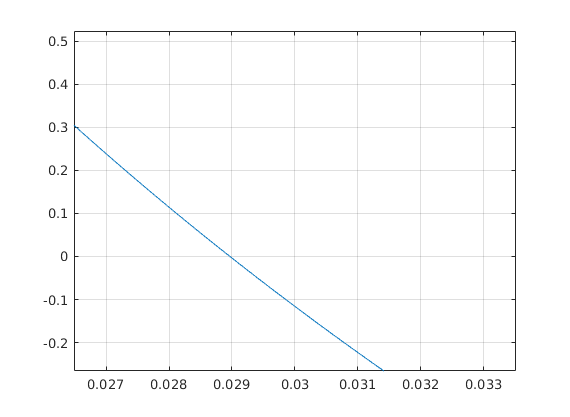
\includegraphics[scale=0.6]{untitled.png}
    
    \subsection{Bisection method and False position method}
    For both of these methods, we approximate the value of the friction factor by using a = 0.008 and b = 0.08, with a tolerance of ${10^{-8}}$
    \subsubsection{Bisection method}
    Took 26 iterations to calculate the answer. The method converges to 0.02896781 
    \subsubsection{False position method}
    Took 31 iterations to calculate the answer. The method converges to 0.02896782
    \subsubsection{Discussion}
    We see that both method converges to the solution, however the bisection method is faster in this case.
    \subsection{Newton's method}
    We can calculate the derivative of the function quite easily: \\
    \[ h'(f) = \frac{-1}{2 f \sqrt{f}} + 2.0 \left(\frac{log_{10} e \times \frac{-2.51}{2 \textit{Re} f \sqrt{f}}}{\frac{\varepsilon}{3.7D} + \frac{2.51}{\textit{Re}\sqrt{f}}}\right) \]\\
    This is then used for the calculation for Newton's method in the Matlab file.
    \subsubsection{With initial guess 0.008}
    Took 6 iteration to calculate the answer. The method converges to 0.02896781 
    \subsubsection{With initial guess 0.08}
    The approximations do not converge. They fluctuate and eventually go to infinity
    \subsubsection{Discussion}
    We see that Newton's method converges extremely fast if we choose the correct initial guess. This is due to the nature of the function around the root.
    \subsection{Using fzero}
    We use the built-in fzero function with options = optimset('Display','iter', 'TolX', 1e-8).This function searches for a point near the guess where the sign of the function changes
    \subsubsection{With initial guess 0.008}
    The method does not converge to the solution. Complex function value encountered during search
    \subsubsection{With initial guess 0.08}
    The method manages to find an interval [0.0288, 0.116204] where the function changes sign. It then continues to search for the root by evaluating possible values in this interval, and eventually got to f = 0.0289678 
    \subsubsection{Discussion}
    As opposed to Newton's method, fzero was able to find the root with initial guess 0.08, but was unable to do so with initial guess 0.008.
    \subsection{Fixed Point Iteration}
    \subsubsection{Iteration function}
    One of the possible iteration functions is: \\
    \[ g(f) = \left(\frac{1}{2.0 \log_{10} \left(\frac{\varepsilon}{3.7D} + \frac{2.51}{\textit{Re}\sqrt{f}}\right)}\right)^2 \]
    \subsubsection{Cobweb Diagrams}
    For initial guess f = 0.008: \\
    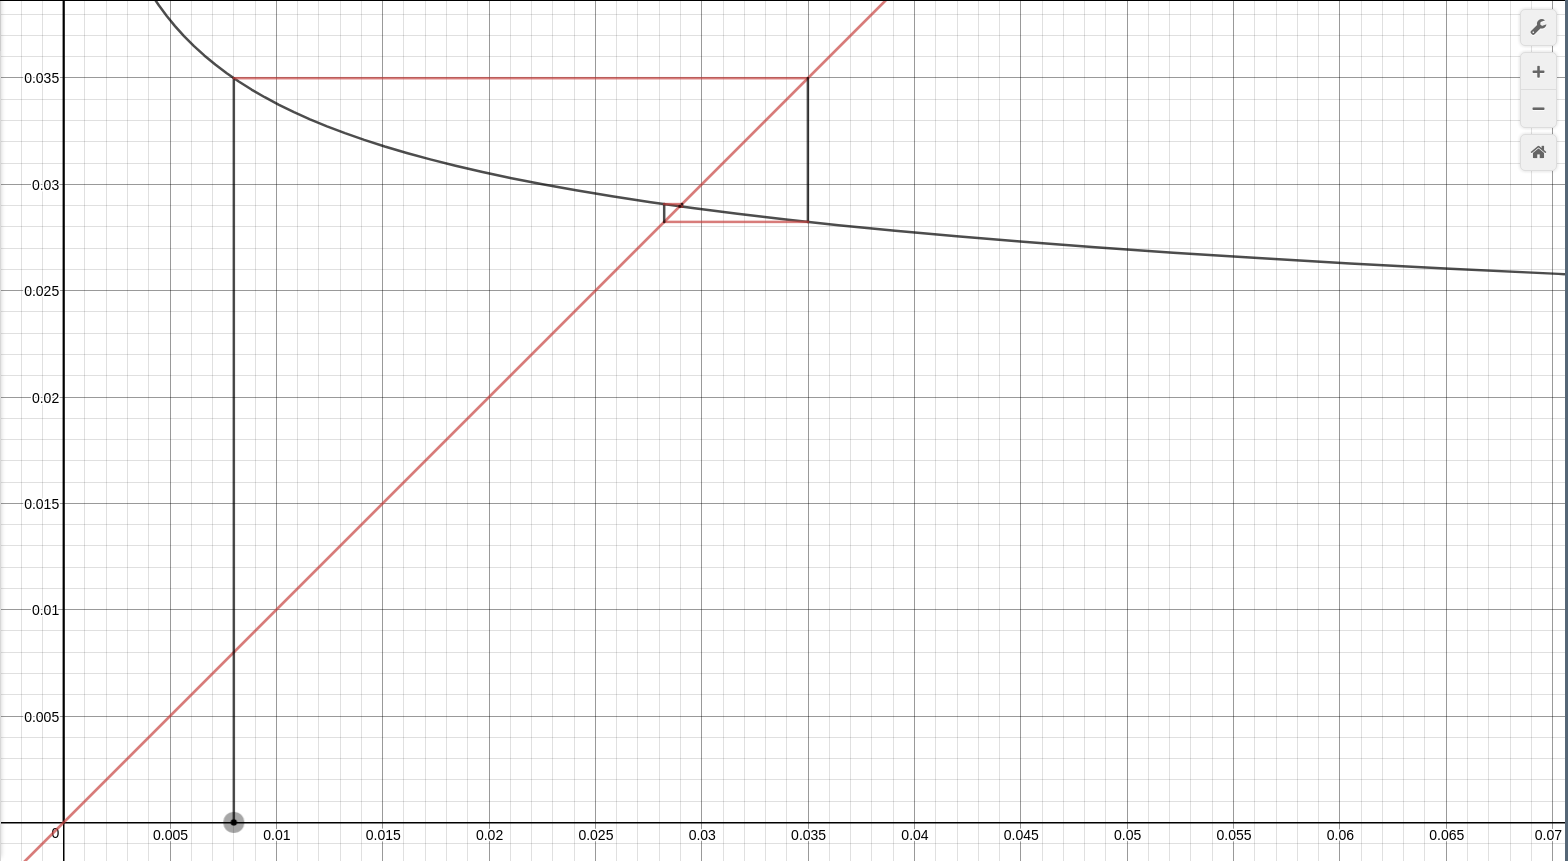
\includegraphics[scale=0.2]{second.png}\\
    For initial guess f = 0.08: \\
    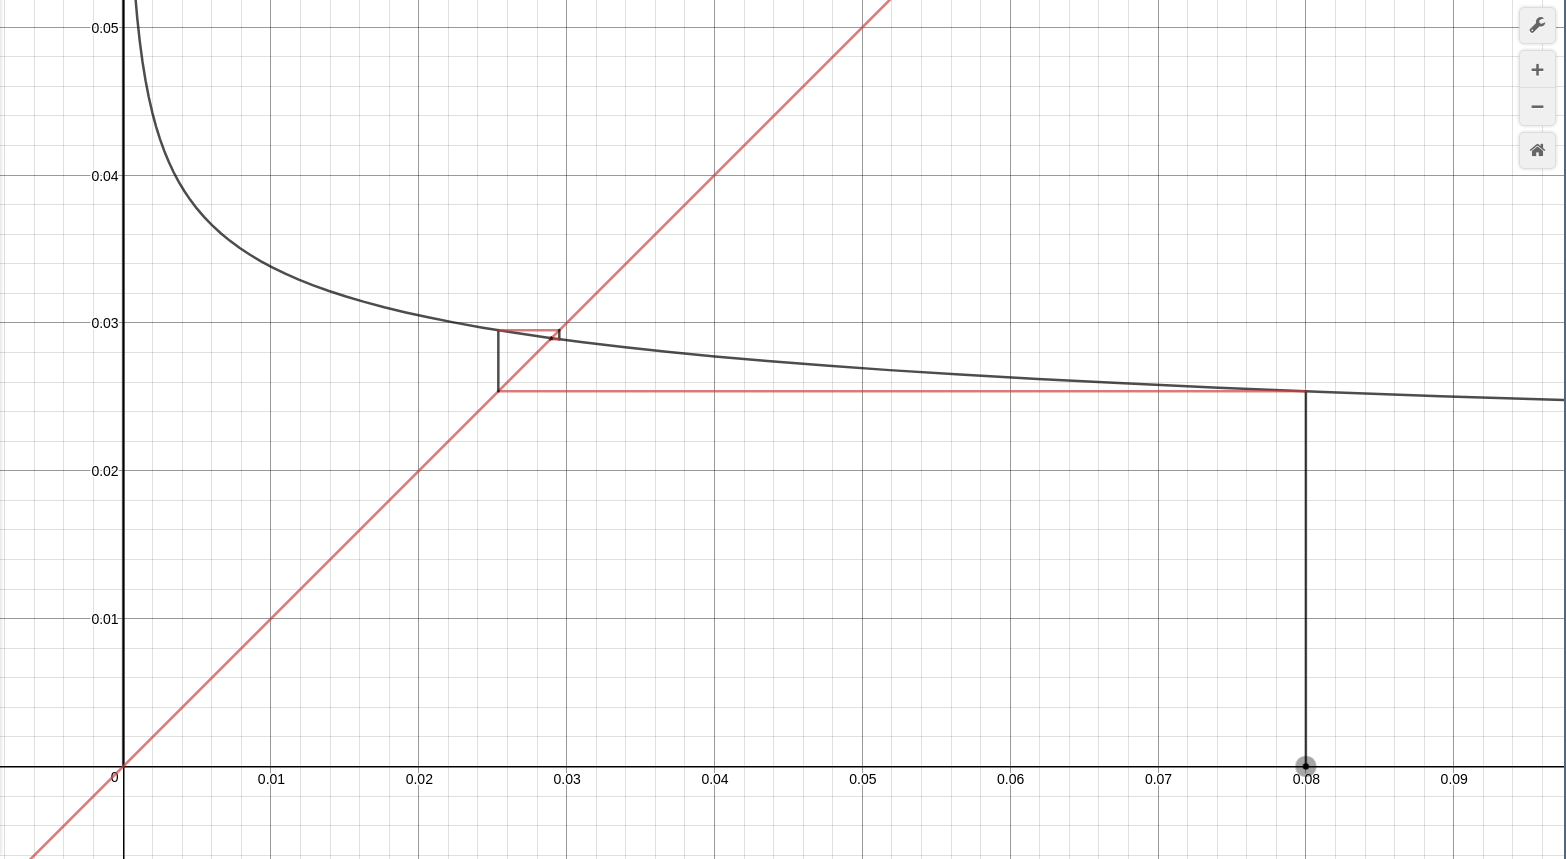
\includegraphics[scale=0.2]{first.png}\\
    \subsection{Discussion}
    With both initial guesses at 0.008 and 0.08, the method was able to find the approximation in 9 iterations. This is because ${|g'(x)| < 1}$ at the root and therefore guarantees convergence.
	
\end{document}